\documentclass[11pt,a4paper]{article}
\usepackage[margin=2cm]{geometry}
\usepackage[T1]{fontenc}
\usepackage[utf8]{inputenc}
\usepackage{lmodern}
\usepackage{microtype}
\usepackage{amsmath}
\usepackage{booktabs}
\usepackage{graphicx}
\usepackage{float}
\usepackage[font=small,labelfont=bf]{caption}
\usepackage{subcaption}
\usepackage{xcolor}
\usepackage{enumitem}
\usepackage[hidelinks]{hyperref}

\graphicspath{{../reports/figures/}{figures/}}
\setlist{nosep,leftmargin=*}
\newcommand{\code}[1]{\texttt{\small #1}}
\emergencystretch=3em % let lines with long code names stretch instead of overflowing

\title{\textbf{Who will be back within 30 days?}\\[2pt]
\large Predicting early readmission of diabetic inpatients to plan hospital beds}
\author{Muhammad TALHA \and Jules BORDAIS \and Elimane DIALLO\\[4pt]
\small Supervised Learning \& Model Engineering --- Fall 2026}
\date{}

\begin{document}
\maketitle

\noindent\fbox{\parbox{\dimexpr\linewidth-2\fboxsep-2\fboxrule}{\small
\textbf{Dataset:} Diabetes 130-US hospitals 1999--2008 (OpenML id 4541), 101{,}766 encounters, 71{,}518 patients.\\
\textbf{Repository:} \url{https://github.com/Elimane29/supervised_learning_project_Muhammad_Jules_Elimane}\\
\textbf{Entry points:} \code{scripts/01\_eda.py} \dots\ \code{09\_leakage\_checks.py}, \code{api/app.py}.}}

\section{Problem framing}

A hospital whose beds are under pressure wants to know, \emph{at discharge}, which diabetic inpatients will be readmitted within 30 days, so that it can plan beds and target follow-up calls. The prediction unit is one encounter; the prediction is made at discharge, so every feature must pass the \emph{prediction-time test}: could its value be known at that moment?

The original target has three classes (\code{NO}, \code{>30}, \code{<30}). We define $Y=1$ for \code{<30} and $Y=0$ otherwise: a return after 30 days does not strain this month's beds. The model estimates $p(x)=P(Y=1\mid x)$; it produces a risk, not a decision. Two downstream uses follow, and they shape our evaluation:
\begin{enumerate}
\item \textbf{Bed planning} uses the \emph{sum} of probabilities, so probabilities must be calibrated (Section~\ref{sec:calib}).
\item \textbf{Follow-up} uses a threshold on $p(x)$, chosen from the relative cost of the two errors (Section~\ref{sec:decision}).
\end{enumerate}
With a positive rate of 11.4\%, a model that always predicts ``no'' reaches 88.6\% accuracy and is useless. Our selection metric is therefore the \textbf{average precision} (AP, the step-wise PR-AUC), whose random baseline equals the prevalence (0.114). We also report ROC-AUC (ranking), the Brier score and the expected calibration error (ECE) (probability quality), and, at the decision threshold, accuracy, precision, recall, F1 and the expected cost. Accuracy is shown for completeness, not for selection: on this data it rewards the model that never flags anyone.

\section{Data understanding and leakage audit}
\label{sec:eda}

\paragraph{Cohort.} Starting from 101{,}766 encounters (71{,}518 patients), we remove 2{,}423 encounters ending in death or hospice and 3 encounters with gender \code{Unknown/Invalid}; the two groups do not overlap. The modelling cohort therefore has $101{,}766 - 2{,}423 - 3 = 99{,}340$ encounters from 69{,}987 patients.

The EDA (\code{scripts/01\_eda.py}, on the development split only) produced seven findings, each turned into a rule (Table~\ref{tab:audit}).

\begin{table}[H]
\centering\small
\begin{tabular}{p{5.2cm}p{2.4cm}p{7.6cm}}
\toprule
Finding & Risk & Decision \\
\midrule
2{,}423 encounters end in death or hospice (discharge ids 11, 13, 14, 19, 20, 21) & target leakage & Removed: these patients cannot be readmitted; keeping them teaches a trivially true, useless rule. \\
3 encounters with gender \code{Unknown/Invalid} & data quality & Removed: too few to learn from, and they would form an empty group in the fairness audit. \\
23\% of patients have several encounters (up to 40) & group leakage & \code{StratifiedGroupKFold} on \code{patient\_nbr} for the test split and every CV fold. \\
Earlier stays of a patient are informative & temporal leakage & History features count only encounters with a smaller \code{encounter\_id}, never later ones. \\
\code{weight} 97\% missing; \code{examide}, \code{citoglipton} constant & noise & Dropped. ``\code{?}'' kept as an explicit \code{Unknown} category: missingness may carry signal (e.g.\ no payer recorded). \\
Admission/discharge ids and age brackets stored as codes & semantics & Ids treated as categories; age bracket mapped to its midpoint (ordinal kept). \\
\code{race} is a sensitive attribute & fairness & Never a model input; kept only for the audit (Section~\ref{sec:fair}). \\
\bottomrule
\end{tabular}
\caption{Data audit: from EDA findings to modelling rules.}
\label{tab:audit}
\end{table}

\begin{figure}[H]
\centering
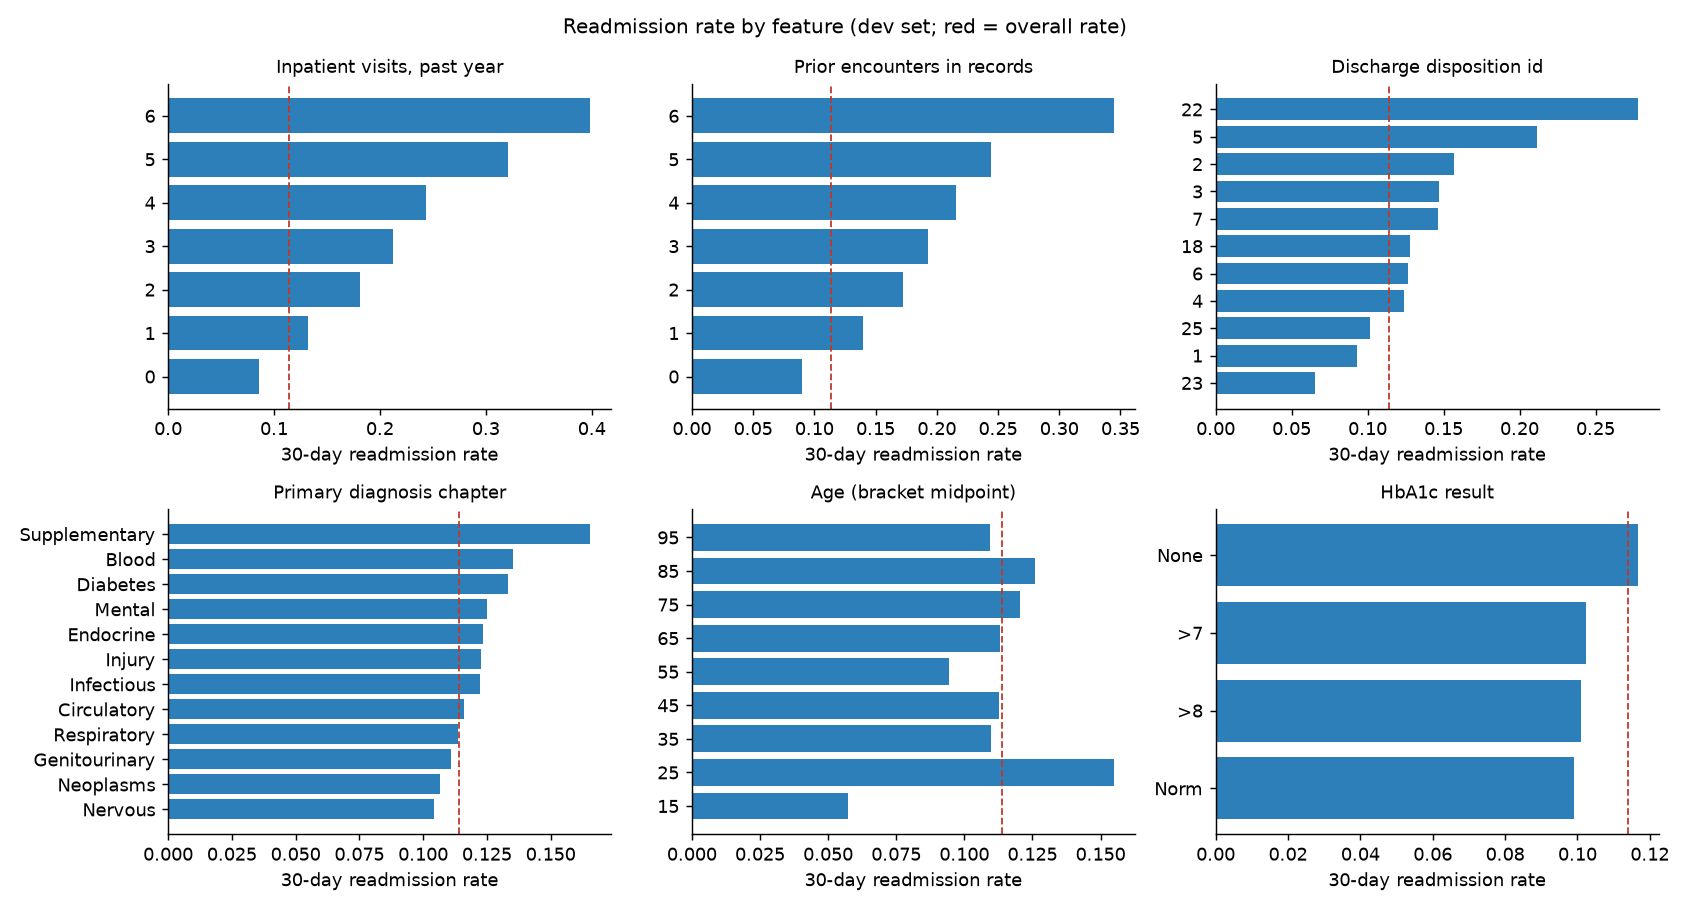
\includegraphics[width=0.72\linewidth]{eda_signal.png}
\caption{30-day readmission rate by feature on the development split (red: overall 11.4\%). Prior hospital use is the strongest univariate signal: from 8.5\% with no inpatient visit in the past year to 40\% with six. Patients without an HbA1c measurement are readmitted more often.}
\label{fig:eda}
\end{figure}

The numeric variables overlap heavily between the two classes (mean length of stay 4.3 vs 4.8 days), except prior utilisation: mean inpatient visits 0.56 vs 1.23 and mean prior encounters 0.55 vs 1.24. This already suggests a hard problem: much of what drives a readmission (adherence, social support) happens after discharge and is not recorded.

\paragraph{Measuring the leaks.} To show what the audit protects against, \code{scripts/09\_leakage\_checks.py} rebuilds the leaky variants on purpose and evaluates them with the same LightGBM and the same metrics on the development set (Table~\ref{tab:leaks}).

\begin{table}[H]
\centering\small
\begin{tabular}{llcc}
\toprule
Check & Variant & CV-val.\ AP $\pm$ sd & CV-val.\ ROC-AUC \\
\midrule
Temporal & history = earlier stays only (ours) & 0.238 $\pm$ 0.012 & 0.685 \\
Temporal & history = earlier + later stays (leaky) & 0.315 $\pm$ 0.010 & 0.789 \\
Temporal & history = later stays only (leaky) & 0.337 $\pm$ 0.008 & 0.800 \\
\midrule
Group & folds grouped by patient (ours) & 0.238 $\pm$ 0.012 & 0.685 \\
Group & patients mixed across folds (leaky) & 0.240 $\pm$ 0.005 & 0.686 \\
\bottomrule
\end{tabular}
\caption{Leaky variants rebuilt on purpose: CV-validation scores, mean $\pm$ sd over the 5 development folds. A higher score for a leaky variant is not a better model: the future is unknown at discharge.}
\label{tab:leaks}
\end{table}

The temporal leak is large. Counting a patient's later stays would raise AP from 0.238 to 0.315, and to 0.337 when only later stays are counted. That is a 32--42\% inflation, and it would vanish in production, because a later stay is often the readmission itself.

The group leak is small here: 0.240 vs 0.238, within one fold standard deviation, although patients were shared between the CV-train and CV-validation parts 27{,}052 times. The model has no patient identifier and only weak patient-specific signals, so it cannot memorise individuals. We keep the grouped split anyway: it is the correct design for new patients, and it costs nothing.

\section{Validation protocol}
\label{sec:protocol}

The cohort is split once with \code{StratifiedGroupKFold} (no patient shared, prevalence 11.39\% on both sides). Throughout the report the sets are named as follows:
\begin{itemize}
\item \textbf{Development set} (80\%, 79{,}473 encounters): everything used to build the model. It is cut into 5 patient-grouped, stratified folds, materialised once and reused by \emph{every} model and Optuna trial, so all comparisons are paired.
\item \textbf{CV-train / CV-validation}: in each of the 5 cross-validation rounds, the Pipeline is fitted on 4 folds (the \emph{CV-train} part, about 63{,}600 encounters) and scored on the 5th (the \emph{CV-validation} part, about 15{,}900). A \emph{CV-validation score} is the mean $\pm$ standard deviation over the 5 rounds; the \emph{out-of-fold predictions} are the 5 CV-validation predictions put together, one per development encounter, never made by a model that saw that encounter.
\item \textbf{Training of the final model}: the frozen Pipeline is refitted once on the whole development set.
\item \textbf{Test set} (20\%, 19{,}867 encounters): held out and scored \textbf{once}, after every choice was frozen.
\end{itemize}
CV-validation scores and out-of-fold predictions are the single source for every decision: model comparison, hyperparameters, calibrator, decision threshold and fairness thresholds. Every score in this report is labelled with the phase it comes from: \emph{CV-validation} (development) or \emph{test}.
\code{TimeSeriesSplit} was rejected: the data have no admission date, and encounter order alone does not define a deployment time. Nested CV was considered; with 80k development rows, CV tuning plus one untouched test set gives an honest estimate at a fraction of the cost (five times fewer fits).

\section{Feature engineering and pipeline}
\label{sec:features}

All features are built by a scikit-learn transformer, \code{ReadmissionFeatures}, so that its only learned rule (which categories are too rare, $<50$ occurrences, and are pooled into \code{Other}) is learned on the training part of each fold. Engineered features:
\begin{itemize}
\item \code{n\_prior\_encounters}: earlier stays of the patient in the records (past only, see Table~\ref{tab:audit}); \code{total\_prior\_visits}: outpatient + emergency + inpatient visits in the past year.
\item ICD-9 chapters for \code{diag\_1/2/3}: about 700 codes mapped to 19 clinical groups (CDC/CMS ranges, with 250.xx split out as \emph{Diabetes}); \code{diabetes\_primary} flags a primary diabetic diagnosis.
\item Treatment complexity: \code{n\_meds\_active} (diabetes drugs taken) and \code{n\_meds\_changed} (dose up or down); care intensity: \code{meds\_per\_day}, \code{labs\_per\_day}.
\item \code{a1c\_tested}, \code{glucose\_tested}: whether the test was done at all (``None'' means not measured).
\end{itemize}

\paragraph{Missing values, without leakage.} The data contain no NaN: missing entries appear as the string ``\code{?}'' in five categorical columns. Mapping ``\code{?}'' to an explicit \code{Unknown} category is a fixed relabelling that learns nothing from the data, so it cannot leak whenever it is applied. The only learned imputation, the numeric median, sits inside the Pipeline. It is therefore fitted on the CV-train part of each fold, and on the full development set for the final model, never on CV-validation or test rows. It is a safeguard for API inputs, since no numeric value is missing in the dataset. A unit test (\code{test\_imputer\_learns\_from\_training\_rows\_only}) checks that the median comes from the training rows only and is not refitted on new rows.

The \textbf{Pipeline} (\code{src/readmission/pipelines.py}) chains \code{ReadmissionFeatures} $\rightarrow$ a \code{ColumnTransformer} $\rightarrow$ the model. Numeric features: median imputation (plus standardisation for the regularised logistic regression). Low-cardinality categoricals: one-hot encoding. The raw ICD-9 codes (high cardinality) are additionally target-encoded with scikit-learn's \code{TargetEncoder}, which \emph{cross-fits} during \code{fit\_transform}: a training row is never encoded with its own label, and rare codes are shrunk towards the mean. CatBoost receives the raw categories instead and encodes them itself with ordered target statistics. We use an \code{imblearn} Pipeline so that a resampler, when tested, acts only at fit time on the training fold. The deployed object is the fitted Pipeline plus calibrator plus threshold, loaded by the API.

\begin{table}[H]
\centering\small
\begin{tabular}{lcc}
\toprule
LightGBM & CV-val.\ AP & CV-val.\ ROC-AUC \\
\midrule
Full feature set & 0.238 & 0.685 \\
$-$ prior encounters & 0.237 & 0.681 \\
$-$ target encoding of ICD-9 codes & 0.238 & 0.682 \\
$-$ both & 0.236 & 0.677 \\
\bottomrule
\end{tabular}
\caption{Feature ablation. The two additions give +0.009 ROC-AUC together; on AP the gain is smaller than the fold standard deviation ($\pm$0.012). We keep them: cheap, clinically meaningful and available at discharge.}
\label{tab:ablation}
\end{table}

\section{Class imbalance}
\label{sec:imbalance}

We compared remedies at three stages (Session 6) with LightGBM on the same folds; all resampling ran inside the training folds only.

\begin{table}[H]
\centering\small
\begin{tabular}{lccc}
\toprule
Remedy (LightGBM) & CV-val.\ AP & CV-val.\ ROC-AUC & CV-val.\ Brier \\
\midrule
None & 0.238 & 0.685 & \textbf{0.095} \\
Class weight $\sqrt{n_0/n_1}=2.8$ & \textbf{0.239} & 0.686 & 0.113 \\
Class weight $n_0/n_1=7.8$ & 0.235 & 0.683 & 0.202 \\
Random undersampling to 1:2 & 0.227 & 0.679 & 0.140 \\
Random oversampling to 1:2 & 0.235 & 0.683 & 0.132 \\
Logistic regression, none $\rightarrow$ \code{balanced} & 0.218 $\rightarrow$ 0.218 & 0.668 $\rightarrow$ 0.670 & 0.097 $\rightarrow$ 0.224 \\
\bottomrule
\end{tabular}
\caption{Imbalance remedies: CV-validation scores on the development set; resampling applied to the CV-train part only.}
\label{tab:imbalance}
\end{table}

No remedy improved the ranking beyond fold noise, and all of them inflated the predicted probabilities (Brier up to 0.20): re-weighting changes the training objective so that $p(x)$ no longer estimates the true frequency. Since our users read the probabilities, we chose to (i) measure with AP rather than accuracy, (ii) leave the class weight to Optuna as a hyperparameter rather than impose it, and (iii) handle the imbalance at the \emph{decision} level with a cost-based threshold on calibrated probabilities, the least invasive remedy. SMOTE was not used: most inputs are categorical, and interpolating between diagnosis codes has no meaning.

\section{Models, tuning and experiment tracking}
\label{sec:models}

We trained four model families of increasing flexibility, all inside the same Pipeline and evaluated on the same folds with the same metrics: a regularised logistic regression (interpretable linear baseline), a Random Forest (bagging of decorrelated trees), LightGBM and CatBoost (gradient boosting).

\paragraph{Optuna.} Each family was tuned with Optuna (\code{scripts/03\_tune.py}): the objective is the mean CV-validation AP over the 5 patient-grouped development folds, the full Pipeline is refitted in every fold, and the test set is never loaded. The TPE sampler proposes configurations from past trials; a median pruner stops a trial after a fold whose running mean is below the median of earlier trials. Search spaces covered regularisation ($C$, L1 vs L2), tree depth and leaves, learning rate jointly with the number of trees, row and column subsampling, and class weights. Elastic Net was excluded after measuring that the required \code{saga} solver was six times slower for the same AP. Budgets: LightGBM 32 trials, logistic 25, Random Forest 15, CatBoost 2 (each CatBoost fit takes about 2.5 minutes per fold; the 40-minute budget allowed two trials).

\paragraph{MLflow.} Every run is logged in an MLflow tracking store (\code{mlflow.db}): one run per untuned experiment (17), one parent run per Optuna study with one nested child run per trial (parameters, per-fold AP and ROC-AUC, mean and standard deviation), and a final run holding the test metrics, figures, tables and the frozen model bundle. The 123 runs are exported to \code{reports/tables/mlflow\_runs.csv}.

\begin{table}[H]
\centering\small
\resizebox{\linewidth}{!}{%
\begin{tabular}{lccccl}
\toprule
Model & CV-val.\ AP untuned & CV-val.\ AP tuned $\pm$ sd & CV-val.\ ROC-AUC & CV-val.\ Brier & Gain \\
\midrule
Dummy (prevalence) & 0.114 & --- & 0.500 & 0.101 & floor \\
Logistic regression (L1, $C=0.21$) & 0.218 & 0.219 $\pm$ 0.012 & 0.670 & 0.097 & linear signal, $\times$1.9 the floor \\
Random Forest & 0.227 & 0.227 $\pm$ 0.014 & 0.681 & 0.096 & +0.008: thresholds, interactions \\
LightGBM & 0.238 & 0.239 $\pm$ 0.013 & 0.686 & 0.097 & +0.012: sequential corrections \\
\textbf{CatBoost} & 0.248 & \textbf{0.248 $\pm$ 0.015} & \textbf{0.688} & \textbf{0.095} & +0.009: ordered categorical encoding \\
\bottomrule
\end{tabular}}
\caption{Model progression: CV-validation scores on the development set (mean over the 5 folds; tuned models re-evaluated on the same folds).}
\label{tab:models}
\end{table}

Each step of the progression bought about +0.01 AP; tuning bought almost nothing ($\leq$0.001), and when the class weight was a free hyperparameter Optuna chose none (logistic, Random Forest, CatBoost) or 1.4 (LightGBM), consistent with Section~\ref{sec:imbalance}. The largest lever was how the high-cardinality categoricals (ICD-9 codes, specialty, discharge disposition) are represented, not the hyperparameters. CatBoost and LightGBM differ by less than one fold standard deviation; CatBoost also has the best Brier score, so it is the final model (iterations 900, depth 7, learning rate 0.067, $\ell_2$ = 1.06, no class weight). The best-of-$N$ CV-validation score is slightly optimistic by construction, which is why the number we report for the final model comes from the test set.

\begin{table}[H]
\centering\small
\resizebox{\linewidth}{!}{%
\begin{tabular}{llcccccccc}
\toprule
 & & & & \multicolumn{2}{c}{$t=0.5$} & \multicolumn{4}{c}{$t=0.175$ (deployed)} \\
\cmidrule(lr){5-6}\cmidrule(lr){7-10}
Phase & Model & ROC-AUC & AP & Accuracy & F1 & Accuracy & Precision & Recall & F1 \\
\midrule
CV-validation & Dummy (prevalence) & 0.500 & 0.114 & 0.886 & 0.000 & 0.886 & 0.000 & 0.000 & 0.000 \\
CV-validation & Logistic regression & 0.670 & 0.218 & 0.886 & 0.033 & 0.828 & 0.255 & 0.265 & 0.260 \\
CV-validation & Random Forest & 0.680 & 0.225 & 0.886 & 0.000 & 0.816 & 0.248 & 0.303 & 0.273 \\
CV-validation & LightGBM & 0.686 & 0.238 & 0.886 & 0.041 & 0.721 & 0.205 & 0.507 & 0.292 \\
CV-validation & \textbf{CatBoost} & \textbf{0.688} & \textbf{0.247} & 0.887 & 0.056 & 0.814 & 0.258 & 0.336 & 0.292 \\
\midrule
\textbf{Test} & \textbf{CatBoost (final)} & 0.683 & 0.239 & 0.887 & 0.046 & 0.809 & 0.249 & 0.336 & 0.286 \\
\bottomrule
\end{tabular}}
\caption{All metrics for all models. CV-validation rows use the pooled out-of-fold predictions of the development set (so AP differs slightly from the fold means of Table~\ref{tab:models}); the test row is the final model scored once. Source: \code{scripts/10\_metrics\_table.py}.}
\label{tab:allmetrics}
\end{table}

Table~\ref{tab:allmetrics} shows why accuracy cannot select a model here. At the default threshold 0.5, every model reaches 0.886--0.887 accuracy, exactly the share of non-readmitted patients, because almost nobody is flagged (F1 $\leq$ 0.06). At the deployed threshold, the final model catches a third of readmissions (F1 0.29) while its accuracy \emph{drops} to 0.81, below the model that never flags anyone. Precision and recall make the trade-off visible. At the same threshold, LightGBM flags 28\% of patients (recall 0.51, precision 0.21) against 15\% for CatBoost (recall 0.34, precision 0.26): LightGBM's class weight of 1.4 inflates its probabilities, so one threshold does not mean the same operating point for both. Their F1 is identical (0.29), and CatBoost's calibrated probabilities make its threshold interpretable.

\section{Test-set evaluation and decision threshold}
\label{sec:decision}

\paragraph{Threshold.} With calibrated probabilities, flagging a patient is worth it when $p\cdot C_{FN} > (1-p)\cdot C_{FP}$, i.e.\ $p > C_{FP}/(C_{FP}+C_{FN})$. We assume a missed early readmission (unplanned bed, emergency readmission) costs five times a false alert (one follow-up call or a provisional bed hold): $C_{FN}=5$, $C_{FP}=1$, so the theoretical threshold is $1/6\approx0.167$. A grid search on the out-of-fold (CV-validation) predictions of the development set gives 0.175, which we freeze. The cost curve is flat between 0.15 and 0.20 (expected cost 0.488--0.495 per discharge), so the choice is robust; with $C_{FN}/C_{FP}=3$ or $10$ the rule would move to 0.25 or 0.09.

\begin{figure}[H]
\centering
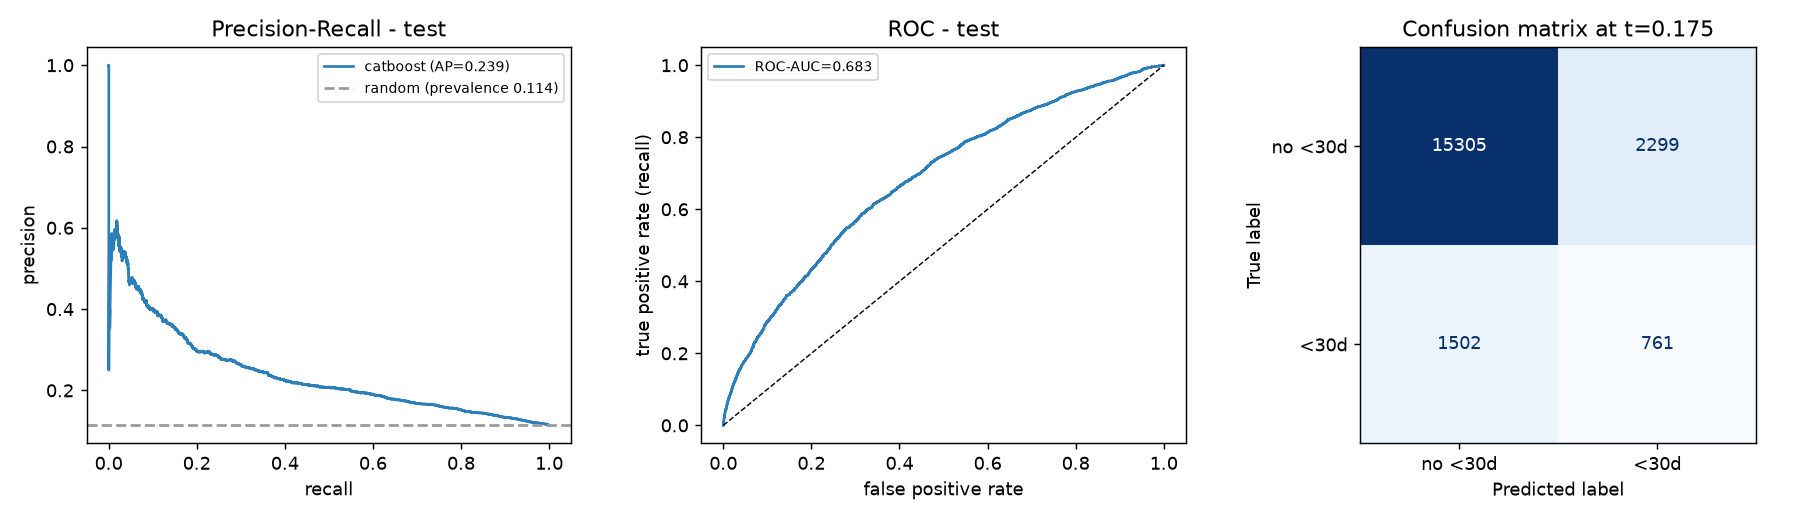
\includegraphics[width=0.85\linewidth]{final_test_curves.png}
\caption{Final CatBoost on the untouched test set: precision--recall curve (AP 0.239 vs 0.114 at random), ROC curve (AUC 0.683) and confusion matrix at $t=0.175$.}
\label{fig:test}
\end{figure}

\begin{table}[H]
\centering\small
\begin{tabular}{lcc}
\toprule
Metric & CV-validation (development) & \textbf{Test (once)} \\
\midrule
Average precision & 0.247 & 0.239 \\
ROC-AUC & 0.688 & 0.683 \\
Brier / ECE & 0.095 / 0.003 & 0.095 / 0.006 \\
Patients flagged at $t=0.175$ & 14.8\% & 15.4\% \\
Recall / precision at $t$ & 0.336 / 0.258 & 0.336 / 0.249 \\
Accuracy / F1 at $t$ & 0.814 / 0.292 & 0.809 / 0.286 \\
TP / FP / FN / TN & --- & 761 / 2{,}299 / 1{,}502 / 15{,}305 \\
Expected cost per discharge & 0.488 & 0.494 \\
\quad baselines: flag nobody / flag all & 0.570 / 0.886 & 0.570 / 0.886 \\
Top 20\% by risk: recall / precision & 0.408 / 0.232 & 0.397 / 0.226 \\
\bottomrule
\end{tabular}
\caption{Final model. The CV-validation and test numbers agree, which supports the protocol: no sign of optimistic selection.}
\label{tab:test}
\end{table}

The model catches one early readmission in three while flagging 15\% of discharges, with alerts 2.2 times more precise than random, and reduces the expected cost by 13\% relative to doing nothing. If follow-up capacity is the binding constraint (e.g.\ 20\% of discharges), ranking by risk catches 40\% of early readmissions. This is a prioritisation tool, not a diagnostic one: published results on this dataset sit in the same ROC-AUC range (0.65--0.70).

\section{Calibration}
\label{sec:calib}

\begin{figure}[H]
\centering
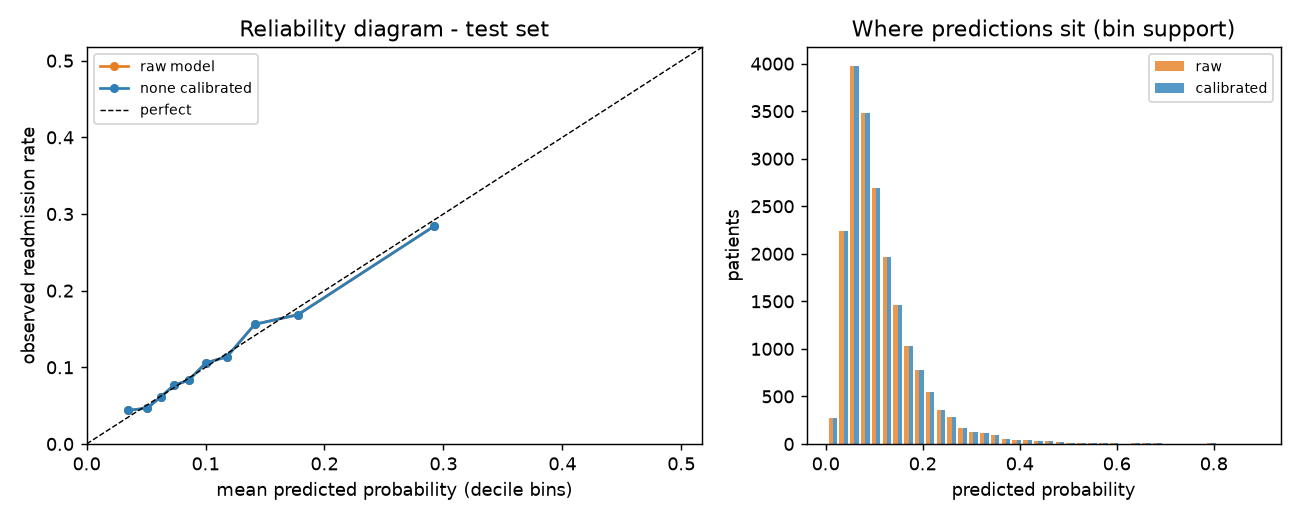
\includegraphics[width=0.7\linewidth]{calibration_test.png}
\caption{Reliability diagram on the test set (quantile bins, so that each point holds 10\% of patients) and distribution of predictions. 89\% of predictions are below 0.2, so uniform bins would leave the upper range almost empty.}
\label{fig:calib}
\end{figure}

The reliability curve follows the diagonal (Figure~\ref{fig:calib}): test Brier 0.095 (0.101 for the base-rate predictor) and ECE 0.006. The model is \textbf{neither over- nor under-confident} overall; the top decile is marginally high (mean prediction 0.29 vs 0.28 observed), within noise for 1{,}987 patients. At the population level, the model expected \textbf{2{,}258 readmissions in the test set; 2{,}263 occurred}.

We compared three options without leakage: for each fold, a calibrator was fitted on the out-of-fold predictions of the other four folds and applied to the CV-validation fold. Platt scaling (on the logit) and isotonic regression did not lower the Brier score (0.0949--0.0950 for all three); isotonic regression lowered the ECE (0.001) but cost AP (0.242 vs 0.247) because its step function ties many scores. We therefore keep the model's probabilities unchanged. The reason it works is the unweighted log-loss training: with class weight 7.8 the Brier score of the same family rises to 0.20 (Table~\ref{tab:imbalance}).

\textbf{Would we trust these probabilities for a downstream decision as-is?} Yes, for bed planning (the sum of probabilities) and for the cost-based threshold, which assumes calibration, on a population like this one. Before deployment we would re-check calibration per hospital and over time, since prevalence and practices drift (the data are from 1999--2008).

\section{Diagnostics: where does the model fail?}
\label{sec:diag}

A good global score can hide failures in important groups (Session 8). We therefore audited the frozen model at the frozen threshold on the test set (\code{scripts/08\_diagnostics.py}). This is an audit only: nothing below was used to change the model. Slices were chosen to be interpretable, large enough and operationally relevant. For each one we report the number of readmissions, the prevalence, recall with a 95\% Wilson interval, and AP relative to the slice's own prevalence.

\begin{table}[H]
\centering\small
\begin{tabular}{lrrcc}
\toprule
Slice (test set, $t=0.175$) & Readmissions & Prevalence & Recall [95\% CI] & AP / prevalence \\
\midrule
Overall & 2{,}263 & 11.4\% & 0.34 & 2.1$\times$ \\
\textbf{No inpatient visit in the past year} & 1{,}127 & 8.6\% & \textbf{0.15} [0.13--0.17] & 2.1$\times$ \\
Discharged home & 1{,}121 & 9.4\% & 0.22 [0.19--0.24] & 2.1$\times$ \\
Age 80+ & 491 & 12.9\% & 0.27 [0.24--0.31] & 1.7$\times$ \\
Two or more inpatient visits & 616 & 21.5\% & 0.72 [0.68--0.75] & 1.5$\times$ \\
Care facility or other hospital & 645 & 16.5\% & 0.52 [0.48--0.56] & 1.8$\times$ \\
\bottomrule
\end{tabular}
\caption{Slice diagnostics. All slices are evaluated with the same model, threshold and period; full table in \code{reports/tables/diagnostics\_slices.csv}.}
\label{tab:slices}
\end{table}

The weakest slice is large and important: \textbf{half of all early readmissions (1{,}127 of 2{,}263) occur in patients without an inpatient visit in the past year, and only 15\% of them are flagged}. The interval [0.13, 0.17] excludes the overall recall, so this is not noise. Within this slice the ranking still works (AP is 2.1 times its prevalence). The failure comes from the global threshold: lower prevalence means lower scores, so few patients cross 0.175.

\paragraph{Error analysis.} Comparing the 1{,}502 missed readmissions (FN) with the 761 caught ones (TP):
\begin{itemize}
\item 64\% vs 22\% had no inpatient visit in the past year;
\item 66\% vs 31\% had no earlier stay in the records;
\item 58\% vs 32\% were discharged home;
\item 48\% of the missed patients received a risk below 0.10.
\end{itemize}
SHAP confirms it. Among actual readmissions, prior inpatient visits contribute +0.32 log-odds on average for TPs and $-$0.02 for FNs; discharge destination contributes +0.27 vs $-$0.02. \emph{Audit finding:} the model relies on utilisation history and treats first-time patients sent home as low risk. \emph{Hypothesis to test:} the information that would reveal their risk (social support, follow-up arrangements) is not recorded. \emph{Next checks:} the same rates among non-readmitted patients, and the same analysis on later data. \emph{Possible actions:} collect post-discharge signals, monitor this slice, or set a slice-specific operating point. No causal claim is made.

\section{Explainability}
\label{sec:shap}

We computed SHAP values with \code{TreeExplainer} on 3{,}000 test patients (log-odds scale, before any calibration; one-hot columns summed back to their feature for the other model families). Global importance (mean $|$SHAP$|$): discharge disposition (0.154), inpatient visits in the past year (0.150), prior encounters (0.083), primary and tertiary ICD-9 codes (0.075, 0.064), total prior visits (0.062), payer code (0.061), age (0.048), primary diagnosis group (0.046) and medical specialty (0.039).

\begin{figure}[H]
\centering
\begin{subfigure}{0.49\linewidth}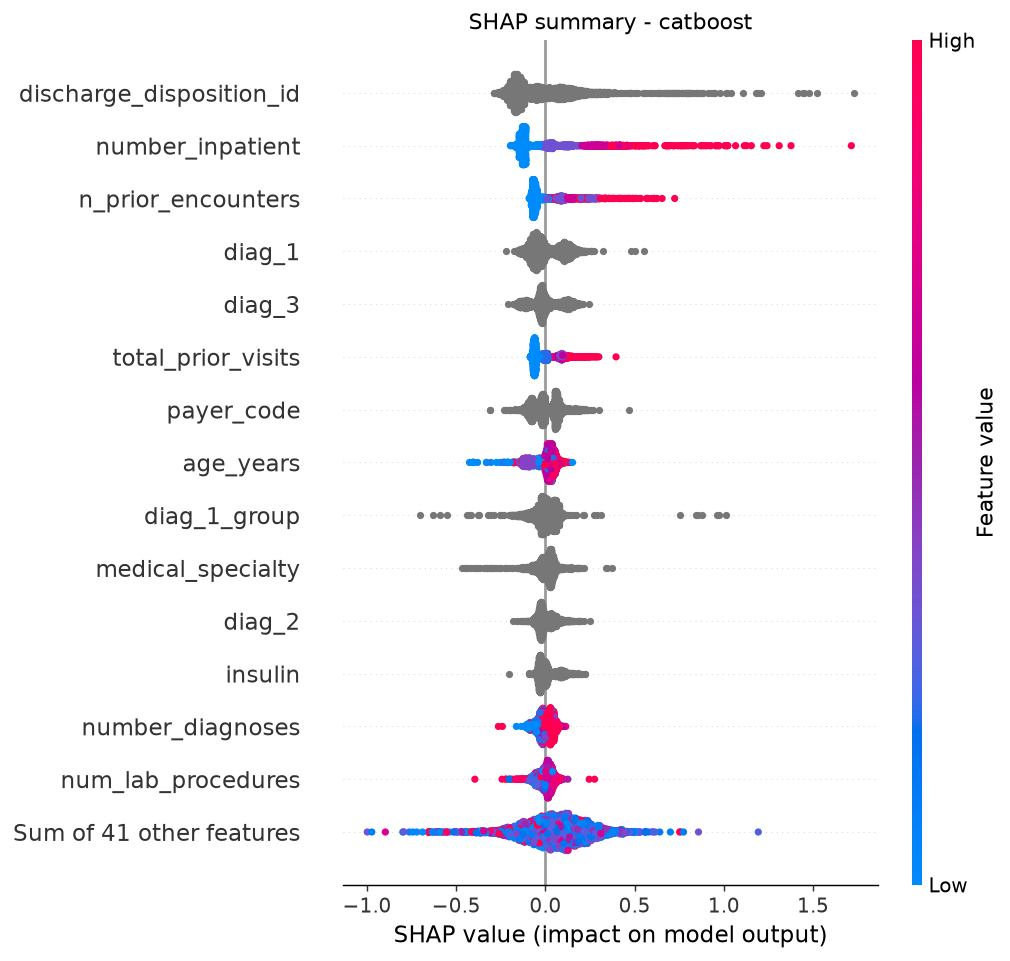
\includegraphics[width=\linewidth]{shap_beeswarm.png}\caption{Global summary (beeswarm).}\end{subfigure}
\hfill
\begin{subfigure}{0.49\linewidth}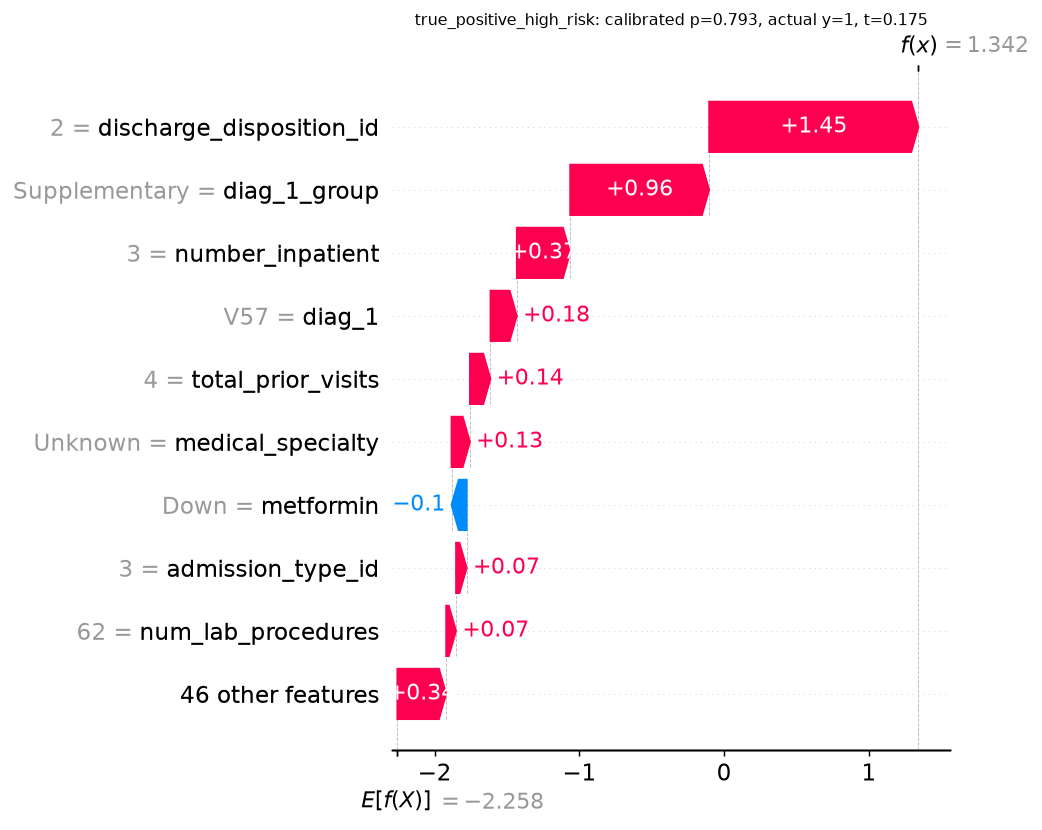
\includegraphics[width=\linewidth]{shap_local_true_positive_high_risk.png}\caption{Highest-risk readmitted patient ($p=0.79$).}\end{subfigure}
\caption{SHAP explanations of the final CatBoost model on test patients.}
\label{fig:shap}
\end{figure}

\paragraph{Business sense.} The ranking matches clinical knowledge. Patients discharged to another facility (skilled nursing, rehabilitation, another hospital) are sicker and less stable; repeated past admissions (``frequent flyers'') are the best-documented readmission predictor. Age matters less than expected: its partial dependence is almost flat (Section~\ref{sec:importance}). The diagnosis codes add case-mix information. Four local explanations are saved (\code{reports/figures/shap\_local\_*.png}). For the highest-risk readmitted patient, disposition (+1.45 log-odds) and primary diagnosis group (+0.96) dominate. The highest-scoring false alert shows the same pattern: the model cannot see what happens after discharge, which caps its precision. The missed readmission ($p=0.02$) had low prior utilisation and a low-risk discharge disposition: nothing in the record announced the return. \textbf{Point of attention:} \code{payer\_code} ranks seventh. Insurance can proxy socio-economic status and, indirectly, race, which motivates the audit below.

\paragraph{Three definitions of importance.}
\label{sec:importance}
Session 8 stresses that importance has no single definition, and our results show why. On the tuned LightGBM, \emph{inpatient visits in the past year} ranks 13th by split count but 2nd by total gain: it is used in few splits, but each one improves the objective a lot. Permutation importance on held-out data (final CatBoost, 6{,}000 test rows, 3 repeats, AP drop) ranks discharge destination (0.053) and inpatient visits (0.032) at the top. Race, which is not an input, has a drop of exactly 0: a sanity check of the method.

Correlated features illustrate the course's warning: inpatient visits and prior encounters have Spearman $\rho=0.74$. Shuffling them one at a time costs 0.032 and 0.009 AP, but shuffling the four history features together costs 0.057, because each feature substitutes for the others.

\paragraph{Partial dependence and ICE.} Setting every patient's number of inpatient visits to the same value and averaging the predictions gives a risk rising from 0.11 (no visit) to 0.30 (seven or more). Length of stay and age are almost flat (0.10--0.12). The ICE curves are roughly parallel, so the average hides no opposite individual responses. Caveat: forcing eight visits on a patient with no prior encounter creates combinations unseen in training. None of these tools is causal: they describe the model, not why patients return.

\begin{figure}[H]
\centering
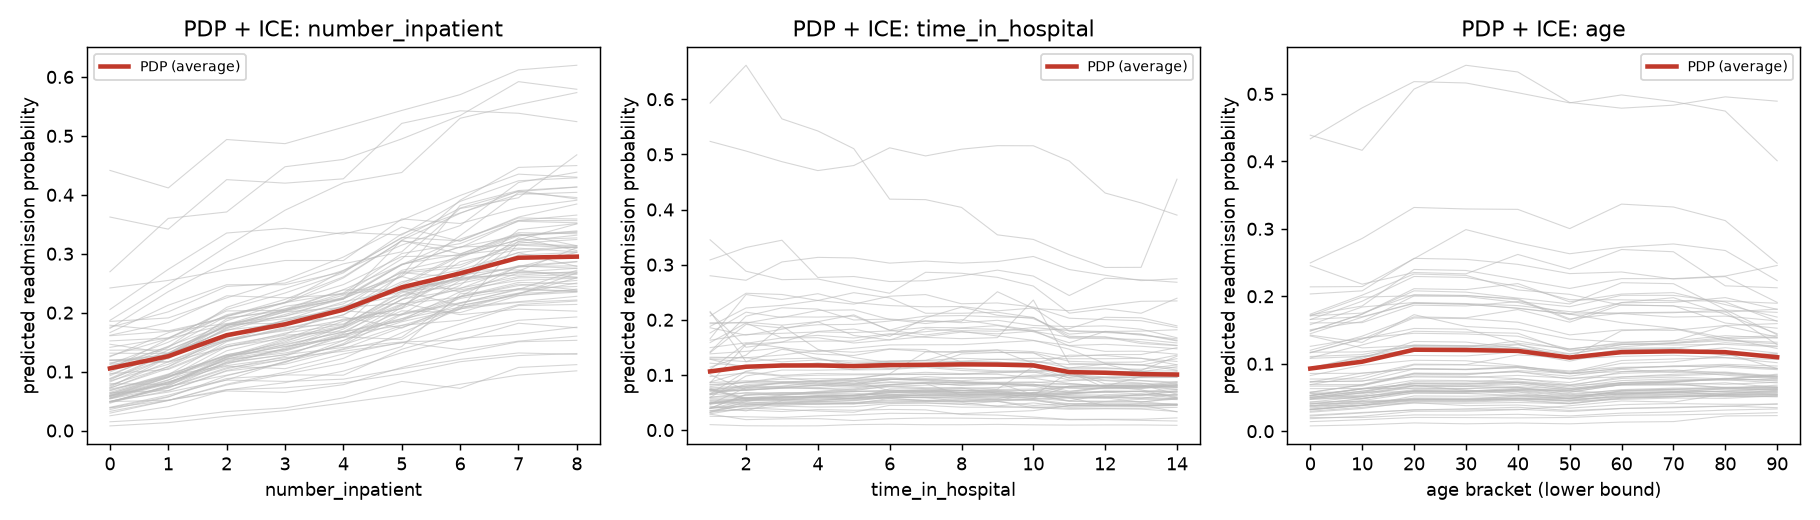
\includegraphics[width=\linewidth]{diagnostics_pdp_ice.png}
\caption{PDP (red) and 80 ICE curves (grey) of the final model on 300 test patients.}
\label{fig:pdp}
\end{figure}

\section{Fairness and bias audit}
\label{sec:fair}

\paragraph{Definition.} We audit race (\code{race}, never used as an input) with \textbf{equal opportunity}: among patients who will be readmitted, the probability of being flagged (the true-positive rate, TPR) should be the same in every group. A flag gives access to follow-up care and a planned bed, so a lower TPR means a group's at-risk patients are more often left without it. Demographic parity (equal flag rates) is reported but not targeted, because base rates genuinely differ (8.0\% for \emph{Unknown} race, 10.2--11.7\% elsewhere). Asian and Other (442 test patients) are merged to keep groups estimable.

\paragraph{Mitigation.} We use post-processing with group-specific thresholds, the deterministic form of fairlearn's \code{ThresholdOptimizer} with a TPR-parity constraint. For each group, the threshold is set on the out-of-fold (CV-validation) predictions of the development set so that its TPR equals the overall CV-validation TPR at $t=0.175$. Thresholds range from 0.127 (\emph{Unknown}) to 0.189 (\emph{Hispanic}). The test set is used only for the before/after comparison.

\begin{figure}[H]
\centering
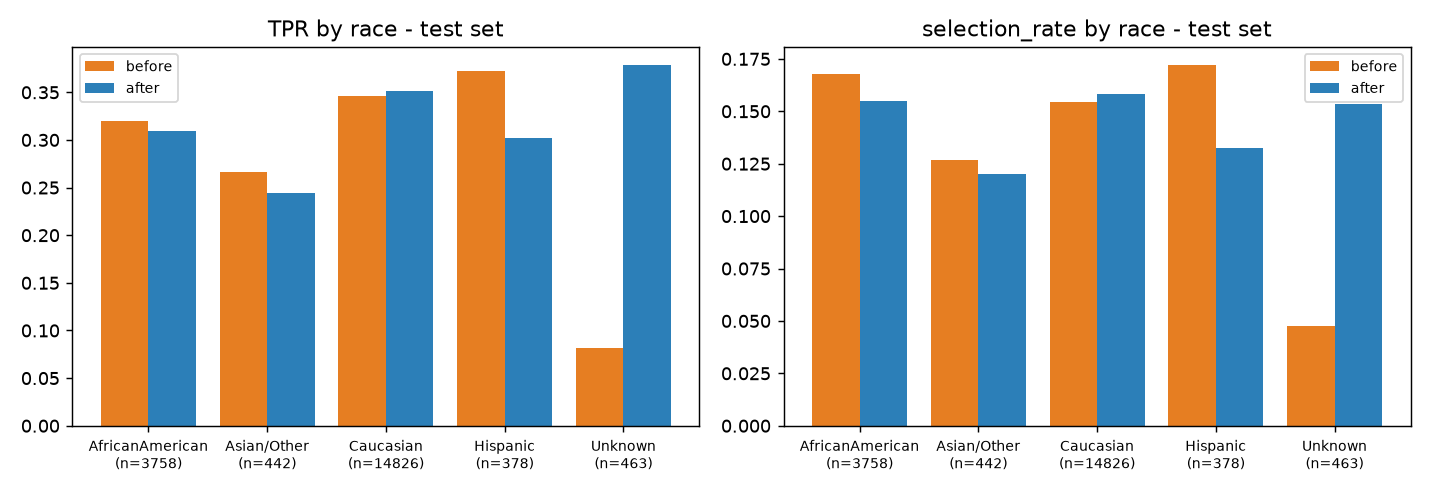
\includegraphics[width=0.8\linewidth]{fairness_race.png}
\caption{TPR and selection rate by race on the test set, before (global threshold) and after (group thresholds).}
\label{fig:fair}
\end{figure}

\begin{table}[H]
\centering\small
\begin{tabular}{lcc}
\toprule
Test set & Before (global $t$) & After (group thresholds) \\
\midrule
Equal opportunity difference (TPR max $-$ min) & 0.291 & \textbf{0.134} \\
Equalized odds difference & 0.291 & 0.134 \\
Demographic parity difference & 0.124 & 0.039 \\
Overall recall / precision & 0.336 / 0.249 & 0.342 / 0.249 \\
Expected cost per discharge & 0.494 & 0.492 \\
\bottomrule
\end{tabular}
\caption{Fairness before and after mitigation (fairlearn \code{MetricFrame}).}
\label{tab:fair}
\end{table}

The mitigation halves the TPR gap at no cost in precision or overall cost. A critical reading is needed, however. The gap is driven by the \emph{Unknown} group, whose TPR rises from 0.08 to 0.38 but which has only 37 readmissions in the test set. Among named groups the gap stays around 0.10 before and after, within the sampling noise of groups with 40--400 positives (standard error $\approx$0.08 for a TPR estimated on 40 positives). Using race at decision time is also a disparate-treatment issue in many jurisdictions. In practice we would keep race out of the decision, monitor TPR by group over time, and investigate why race is missing for some patients (a data-quality signal in its own right). Gender shows no gap (TPR 0.33 vs 0.35); the youngest and oldest age brackets are too small to conclude.

\section{Limitations and conclusion}

\textbf{Limitations.}
\begin{itemize}
\item Performance is modest (AP 0.24, ROC-AUC 0.68): the main drivers of a readmission occur after discharge and are not recorded.
\item The data are 1999--2008 with no dates, so no temporal validation was possible.
\item Costs are assumptions, although the decision rule makes them explicit and the cost curve is flat around the optimum.
\item CatBoost was only lightly tuned, and the target encoder's internal folds are not grouped by patient. That affects only the training-time encoding, never validation.
\item Small racial groups make fairness estimates noisy.
\end{itemize}

\textbf{Conclusion.} We built an end-to-end, leakage-safe supervised-learning system: patient-disjoint validation, all preprocessing fitted per fold, a single test evaluation, Optuna tuning tracked in MLflow, calibrated probabilities, a cost-based decision rule, SHAP explanations, a fairness audit, and a FastAPI endpoint that serves the frozen pipeline.

Model family and the encoding of categoricals bought performance; resampling, class weights and long tuning did not. The final CatBoost model ranks moderately well, but its probabilities are reliable (2{,}258 expected vs 2{,}263 observed readmissions). For a bed-planning use case this matters more than a few points of AUC.

\section*{Use of AI assistants}
Claude (Anthropic) was used as a coding and drafting assistant to help structure the Python package and scripts, support implementation of the experiment pipeline, and draft parts of the slides and report. ChatGPT (OpenAI) was also used to support debugging, conceptual review, interpretation of modelling choices and metrics, and preparation of the presentation.

The exploratory data analysis was carried out by the group, and the course material was studied independently in order to challenge AI-generated coding choices, verify that the modelling decisions were consistent with the concepts taught in class, and check the coherence of the project as a whole. All modelling decisions, validation choices, results and interpretations were reviewed by the group, and every member can explain and defend the final methodology and conclusions.

\appendix
\section{Reproducibility}
\begin{itemize}
\item Environment: Python 3.13, pinned \code{requirements.txt}, \code{pip install -e .}.
\item Order of execution: \code{01\_eda}, \code{02\_experiments}, \code{03\_tune}, \code{04\_finalize}, \code{05\_explain}, \code{06\_fairness}, \code{07\_export\_runs}, \code{08\_diagnostics}, \code{09\_leakage\_checks}.
\item Configuration: every choice lives in \code{configs/config.yaml}, including the cohort exclusions, the CV, the costs, the Optuna budgets and MLflow.
\item Determinism: one seed (42) for all splits, models and samplers.
\item Tests: \code{pytest} (11 tests) covers ICD-9 grouping, the past-only history feature, rare-category pooling learned on fit data only, monotone calibrators, ECE and the API end to end.
\item Serving: \code{uvicorn api.app:app}, then \code{POST /predict} with the encounter's fields; missing fields take the documented defaults.
\end{itemize}

\section{Tuned hyperparameters}
\begin{table}[H]
\centering\small
\begin{tabular}{lp{12.5cm}}
\toprule
Model & Best configuration (mean CV-validation AP) \\
\midrule
Logistic regression & L1, $C=0.213$, no class weight (0.219) \\
Random Forest & 200 trees, max depth 25, min samples leaf 29, max features 0.19, max samples 0.37, no class weight (0.227) \\
LightGBM & 900 trees, learning rate 0.006, 33 leaves, max depth 6, min child samples 27, subsample 0.91, colsample 0.38, $\alpha=0.18$, $\lambda=0.016$, scale\_pos\_weight 1.41 (0.239) \\
CatBoost & 900 iterations, learning rate 0.067, depth 7, $\ell_2$ leaf reg 1.06, no class weight (0.248) \\
\bottomrule
\end{tabular}
\end{table}

\section{Additional figures}
\begin{figure}[H]
\centering
\begin{subfigure}{0.49\linewidth}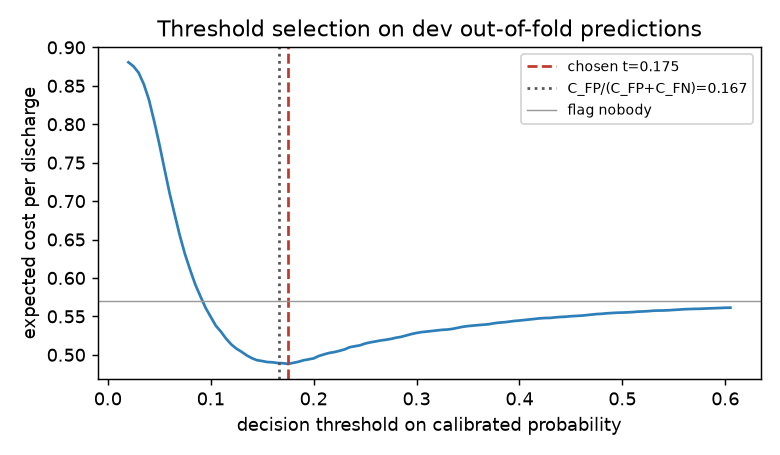
\includegraphics[width=\linewidth]{threshold_cost_curve.png}\caption{Threshold selection on the out-of-fold (CV-validation) predictions.}\end{subfigure}
\hfill
\begin{subfigure}{0.49\linewidth}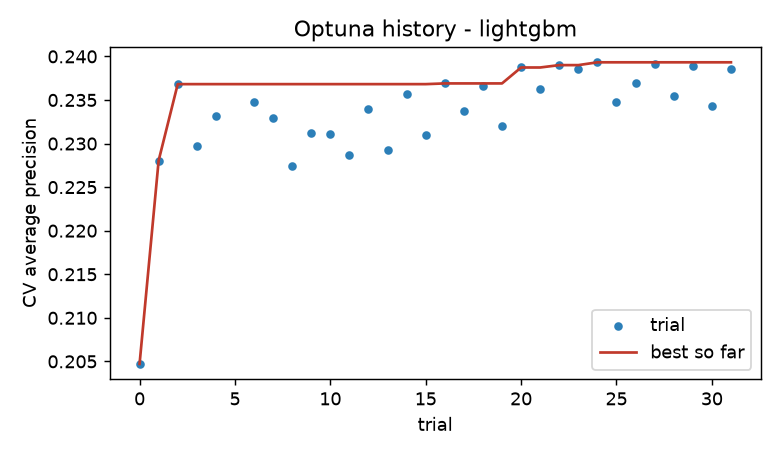
\includegraphics[width=\linewidth]{optuna_history_lightgbm.png}\caption{Optuna history, LightGBM.}\end{subfigure}
\end{figure}
\begin{figure}[H]
\centering
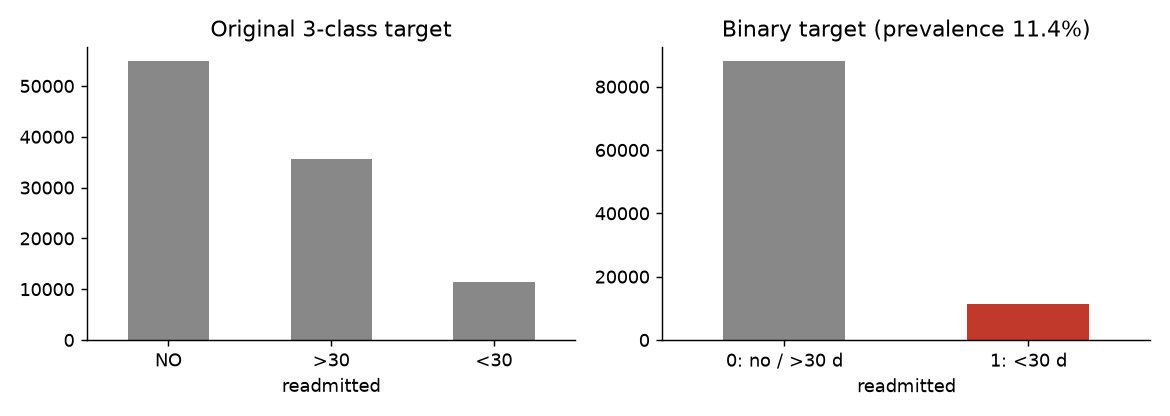
\includegraphics[width=0.75\linewidth]{eda_target.png}
\caption{Original three-class target and binary recoding.}
\end{figure}

\end{document}
